
% Default to the notebook output style

    


% Inherit from the specified cell style.




    
\documentclass[11pt]{article}

    
    
    \usepackage[T1]{fontenc}
    % Nicer default font (+ math font) than Computer Modern for most use cases
    \usepackage{mathpazo}

    % Basic figure setup, for now with no caption control since it's done
    % automatically by Pandoc (which extracts ![](path) syntax from Markdown).
    \usepackage{graphicx}
    % We will generate all images so they have a width \maxwidth. This means
    % that they will get their normal width if they fit onto the page, but
    % are scaled down if they would overflow the margins.
    \makeatletter
    \def\maxwidth{\ifdim\Gin@nat@width>\linewidth\linewidth
    \else\Gin@nat@width\fi}
    \makeatother
    \let\Oldincludegraphics\includegraphics
    % Set max figure width to be 80% of text width, for now hardcoded.
    \renewcommand{\includegraphics}[1]{\Oldincludegraphics[width=.8\maxwidth]{#1}}
    % Ensure that by default, figures have no caption (until we provide a
    % proper Figure object with a Caption API and a way to capture that
    % in the conversion process - todo).
    \usepackage{caption}
    \DeclareCaptionLabelFormat{nolabel}{}
    \captionsetup{labelformat=nolabel}

    \usepackage{adjustbox} % Used to constrain images to a maximum size 
    \usepackage{xcolor} % Allow colors to be defined
    \usepackage{enumerate} % Needed for markdown enumerations to work
    \usepackage{geometry} % Used to adjust the document margins
    \usepackage{amsmath} % Equations
    \usepackage{amssymb} % Equations
    \usepackage{textcomp} % defines textquotesingle
    % Hack from http://tex.stackexchange.com/a/47451/13684:
    \AtBeginDocument{%
        \def\PYZsq{\textquotesingle}% Upright quotes in Pygmentized code
    }
    \usepackage{upquote} % Upright quotes for verbatim code
    \usepackage{eurosym} % defines \euro
    \usepackage[mathletters]{ucs} % Extended unicode (utf-8) support
    \usepackage[utf8x]{inputenc} % Allow utf-8 characters in the tex document
    \usepackage{fancyvrb} % verbatim replacement that allows latex
    \usepackage{grffile} % extends the file name processing of package graphics 
                         % to support a larger range 
    % The hyperref package gives us a pdf with properly built
    % internal navigation ('pdf bookmarks' for the table of contents,
    % internal cross-reference links, web links for URLs, etc.)
    \usepackage{hyperref}
    \usepackage{longtable} % longtable support required by pandoc >1.10
    \usepackage{booktabs}  % table support for pandoc > 1.12.2
    \usepackage[inline]{enumitem} % IRkernel/repr support (it uses the enumerate* environment)
    \usepackage[normalem]{ulem} % ulem is needed to support strikethroughs (\sout)
                                % normalem makes italics be italics, not underlines
    

    
    
    % Colors for the hyperref package
    \definecolor{urlcolor}{rgb}{0,.145,.698}
    \definecolor{linkcolor}{rgb}{.71,0.21,0.01}
    \definecolor{citecolor}{rgb}{.12,.54,.11}

    % ANSI colors
    \definecolor{ansi-black}{HTML}{3E424D}
    \definecolor{ansi-black-intense}{HTML}{282C36}
    \definecolor{ansi-red}{HTML}{E75C58}
    \definecolor{ansi-red-intense}{HTML}{B22B31}
    \definecolor{ansi-green}{HTML}{00A250}
    \definecolor{ansi-green-intense}{HTML}{007427}
    \definecolor{ansi-yellow}{HTML}{DDB62B}
    \definecolor{ansi-yellow-intense}{HTML}{B27D12}
    \definecolor{ansi-blue}{HTML}{208FFB}
    \definecolor{ansi-blue-intense}{HTML}{0065CA}
    \definecolor{ansi-magenta}{HTML}{D160C4}
    \definecolor{ansi-magenta-intense}{HTML}{A03196}
    \definecolor{ansi-cyan}{HTML}{60C6C8}
    \definecolor{ansi-cyan-intense}{HTML}{258F8F}
    \definecolor{ansi-white}{HTML}{C5C1B4}
    \definecolor{ansi-white-intense}{HTML}{A1A6B2}

    % commands and environments needed by pandoc snippets
    % extracted from the output of `pandoc -s`
    \providecommand{\tightlist}{%
      \setlength{\itemsep}{0pt}\setlength{\parskip}{0pt}}
    \DefineVerbatimEnvironment{Highlighting}{Verbatim}{commandchars=\\\{\}}
    % Add ',fontsize=\small' for more characters per line
    \newenvironment{Shaded}{}{}
    \newcommand{\KeywordTok}[1]{\textcolor[rgb]{0.00,0.44,0.13}{\textbf{{#1}}}}
    \newcommand{\DataTypeTok}[1]{\textcolor[rgb]{0.56,0.13,0.00}{{#1}}}
    \newcommand{\DecValTok}[1]{\textcolor[rgb]{0.25,0.63,0.44}{{#1}}}
    \newcommand{\BaseNTok}[1]{\textcolor[rgb]{0.25,0.63,0.44}{{#1}}}
    \newcommand{\FloatTok}[1]{\textcolor[rgb]{0.25,0.63,0.44}{{#1}}}
    \newcommand{\CharTok}[1]{\textcolor[rgb]{0.25,0.44,0.63}{{#1}}}
    \newcommand{\StringTok}[1]{\textcolor[rgb]{0.25,0.44,0.63}{{#1}}}
    \newcommand{\CommentTok}[1]{\textcolor[rgb]{0.38,0.63,0.69}{\textit{{#1}}}}
    \newcommand{\OtherTok}[1]{\textcolor[rgb]{0.00,0.44,0.13}{{#1}}}
    \newcommand{\AlertTok}[1]{\textcolor[rgb]{1.00,0.00,0.00}{\textbf{{#1}}}}
    \newcommand{\FunctionTok}[1]{\textcolor[rgb]{0.02,0.16,0.49}{{#1}}}
    \newcommand{\RegionMarkerTok}[1]{{#1}}
    \newcommand{\ErrorTok}[1]{\textcolor[rgb]{1.00,0.00,0.00}{\textbf{{#1}}}}
    \newcommand{\NormalTok}[1]{{#1}}
    
    % Additional commands for more recent versions of Pandoc
    \newcommand{\ConstantTok}[1]{\textcolor[rgb]{0.53,0.00,0.00}{{#1}}}
    \newcommand{\SpecialCharTok}[1]{\textcolor[rgb]{0.25,0.44,0.63}{{#1}}}
    \newcommand{\VerbatimStringTok}[1]{\textcolor[rgb]{0.25,0.44,0.63}{{#1}}}
    \newcommand{\SpecialStringTok}[1]{\textcolor[rgb]{0.73,0.40,0.53}{{#1}}}
    \newcommand{\ImportTok}[1]{{#1}}
    \newcommand{\DocumentationTok}[1]{\textcolor[rgb]{0.73,0.13,0.13}{\textit{{#1}}}}
    \newcommand{\AnnotationTok}[1]{\textcolor[rgb]{0.38,0.63,0.69}{\textbf{\textit{{#1}}}}}
    \newcommand{\CommentVarTok}[1]{\textcolor[rgb]{0.38,0.63,0.69}{\textbf{\textit{{#1}}}}}
    \newcommand{\VariableTok}[1]{\textcolor[rgb]{0.10,0.09,0.49}{{#1}}}
    \newcommand{\ControlFlowTok}[1]{\textcolor[rgb]{0.00,0.44,0.13}{\textbf{{#1}}}}
    \newcommand{\OperatorTok}[1]{\textcolor[rgb]{0.40,0.40,0.40}{{#1}}}
    \newcommand{\BuiltInTok}[1]{{#1}}
    \newcommand{\ExtensionTok}[1]{{#1}}
    \newcommand{\PreprocessorTok}[1]{\textcolor[rgb]{0.74,0.48,0.00}{{#1}}}
    \newcommand{\AttributeTok}[1]{\textcolor[rgb]{0.49,0.56,0.16}{{#1}}}
    \newcommand{\InformationTok}[1]{\textcolor[rgb]{0.38,0.63,0.69}{\textbf{\textit{{#1}}}}}
    \newcommand{\WarningTok}[1]{\textcolor[rgb]{0.38,0.63,0.69}{\textbf{\textit{{#1}}}}}
    
    
    % Define a nice break command that doesn't care if a line doesn't already
    % exist.
    \def\br{\hspace*{\fill} \\* }
    % Math Jax compatability definitions
    \def\gt{>}
    \def\lt{<}
    % Document parameters
    \title{BattleOfTheNeighborhoods-Report}
    
    
    

    % Pygments definitions
    
\makeatletter
\def\PY@reset{\let\PY@it=\relax \let\PY@bf=\relax%
    \let\PY@ul=\relax \let\PY@tc=\relax%
    \let\PY@bc=\relax \let\PY@ff=\relax}
\def\PY@tok#1{\csname PY@tok@#1\endcsname}
\def\PY@toks#1+{\ifx\relax#1\empty\else%
    \PY@tok{#1}\expandafter\PY@toks\fi}
\def\PY@do#1{\PY@bc{\PY@tc{\PY@ul{%
    \PY@it{\PY@bf{\PY@ff{#1}}}}}}}
\def\PY#1#2{\PY@reset\PY@toks#1+\relax+\PY@do{#2}}

\expandafter\def\csname PY@tok@kn\endcsname{\let\PY@bf=\textbf\def\PY@tc##1{\textcolor[rgb]{0.00,0.50,0.00}{##1}}}
\expandafter\def\csname PY@tok@nd\endcsname{\def\PY@tc##1{\textcolor[rgb]{0.67,0.13,1.00}{##1}}}
\expandafter\def\csname PY@tok@ow\endcsname{\let\PY@bf=\textbf\def\PY@tc##1{\textcolor[rgb]{0.67,0.13,1.00}{##1}}}
\expandafter\def\csname PY@tok@err\endcsname{\def\PY@bc##1{\setlength{\fboxsep}{0pt}\fcolorbox[rgb]{1.00,0.00,0.00}{1,1,1}{\strut ##1}}}
\expandafter\def\csname PY@tok@s2\endcsname{\def\PY@tc##1{\textcolor[rgb]{0.73,0.13,0.13}{##1}}}
\expandafter\def\csname PY@tok@gs\endcsname{\let\PY@bf=\textbf}
\expandafter\def\csname PY@tok@kd\endcsname{\let\PY@bf=\textbf\def\PY@tc##1{\textcolor[rgb]{0.00,0.50,0.00}{##1}}}
\expandafter\def\csname PY@tok@go\endcsname{\def\PY@tc##1{\textcolor[rgb]{0.53,0.53,0.53}{##1}}}
\expandafter\def\csname PY@tok@sx\endcsname{\def\PY@tc##1{\textcolor[rgb]{0.00,0.50,0.00}{##1}}}
\expandafter\def\csname PY@tok@sr\endcsname{\def\PY@tc##1{\textcolor[rgb]{0.73,0.40,0.53}{##1}}}
\expandafter\def\csname PY@tok@gp\endcsname{\let\PY@bf=\textbf\def\PY@tc##1{\textcolor[rgb]{0.00,0.00,0.50}{##1}}}
\expandafter\def\csname PY@tok@vm\endcsname{\def\PY@tc##1{\textcolor[rgb]{0.10,0.09,0.49}{##1}}}
\expandafter\def\csname PY@tok@nc\endcsname{\let\PY@bf=\textbf\def\PY@tc##1{\textcolor[rgb]{0.00,0.00,1.00}{##1}}}
\expandafter\def\csname PY@tok@kr\endcsname{\let\PY@bf=\textbf\def\PY@tc##1{\textcolor[rgb]{0.00,0.50,0.00}{##1}}}
\expandafter\def\csname PY@tok@cs\endcsname{\let\PY@it=\textit\def\PY@tc##1{\textcolor[rgb]{0.25,0.50,0.50}{##1}}}
\expandafter\def\csname PY@tok@sa\endcsname{\def\PY@tc##1{\textcolor[rgb]{0.73,0.13,0.13}{##1}}}
\expandafter\def\csname PY@tok@fm\endcsname{\def\PY@tc##1{\textcolor[rgb]{0.00,0.00,1.00}{##1}}}
\expandafter\def\csname PY@tok@cm\endcsname{\let\PY@it=\textit\def\PY@tc##1{\textcolor[rgb]{0.25,0.50,0.50}{##1}}}
\expandafter\def\csname PY@tok@sc\endcsname{\def\PY@tc##1{\textcolor[rgb]{0.73,0.13,0.13}{##1}}}
\expandafter\def\csname PY@tok@s\endcsname{\def\PY@tc##1{\textcolor[rgb]{0.73,0.13,0.13}{##1}}}
\expandafter\def\csname PY@tok@mb\endcsname{\def\PY@tc##1{\textcolor[rgb]{0.40,0.40,0.40}{##1}}}
\expandafter\def\csname PY@tok@kc\endcsname{\let\PY@bf=\textbf\def\PY@tc##1{\textcolor[rgb]{0.00,0.50,0.00}{##1}}}
\expandafter\def\csname PY@tok@gt\endcsname{\def\PY@tc##1{\textcolor[rgb]{0.00,0.27,0.87}{##1}}}
\expandafter\def\csname PY@tok@il\endcsname{\def\PY@tc##1{\textcolor[rgb]{0.40,0.40,0.40}{##1}}}
\expandafter\def\csname PY@tok@sh\endcsname{\def\PY@tc##1{\textcolor[rgb]{0.73,0.13,0.13}{##1}}}
\expandafter\def\csname PY@tok@ss\endcsname{\def\PY@tc##1{\textcolor[rgb]{0.10,0.09,0.49}{##1}}}
\expandafter\def\csname PY@tok@ni\endcsname{\let\PY@bf=\textbf\def\PY@tc##1{\textcolor[rgb]{0.60,0.60,0.60}{##1}}}
\expandafter\def\csname PY@tok@mi\endcsname{\def\PY@tc##1{\textcolor[rgb]{0.40,0.40,0.40}{##1}}}
\expandafter\def\csname PY@tok@mf\endcsname{\def\PY@tc##1{\textcolor[rgb]{0.40,0.40,0.40}{##1}}}
\expandafter\def\csname PY@tok@nn\endcsname{\let\PY@bf=\textbf\def\PY@tc##1{\textcolor[rgb]{0.00,0.00,1.00}{##1}}}
\expandafter\def\csname PY@tok@mo\endcsname{\def\PY@tc##1{\textcolor[rgb]{0.40,0.40,0.40}{##1}}}
\expandafter\def\csname PY@tok@gr\endcsname{\def\PY@tc##1{\textcolor[rgb]{1.00,0.00,0.00}{##1}}}
\expandafter\def\csname PY@tok@nl\endcsname{\def\PY@tc##1{\textcolor[rgb]{0.63,0.63,0.00}{##1}}}
\expandafter\def\csname PY@tok@o\endcsname{\def\PY@tc##1{\textcolor[rgb]{0.40,0.40,0.40}{##1}}}
\expandafter\def\csname PY@tok@na\endcsname{\def\PY@tc##1{\textcolor[rgb]{0.49,0.56,0.16}{##1}}}
\expandafter\def\csname PY@tok@si\endcsname{\let\PY@bf=\textbf\def\PY@tc##1{\textcolor[rgb]{0.73,0.40,0.53}{##1}}}
\expandafter\def\csname PY@tok@gh\endcsname{\let\PY@bf=\textbf\def\PY@tc##1{\textcolor[rgb]{0.00,0.00,0.50}{##1}}}
\expandafter\def\csname PY@tok@nf\endcsname{\def\PY@tc##1{\textcolor[rgb]{0.00,0.00,1.00}{##1}}}
\expandafter\def\csname PY@tok@c1\endcsname{\let\PY@it=\textit\def\PY@tc##1{\textcolor[rgb]{0.25,0.50,0.50}{##1}}}
\expandafter\def\csname PY@tok@kt\endcsname{\def\PY@tc##1{\textcolor[rgb]{0.69,0.00,0.25}{##1}}}
\expandafter\def\csname PY@tok@vg\endcsname{\def\PY@tc##1{\textcolor[rgb]{0.10,0.09,0.49}{##1}}}
\expandafter\def\csname PY@tok@no\endcsname{\def\PY@tc##1{\textcolor[rgb]{0.53,0.00,0.00}{##1}}}
\expandafter\def\csname PY@tok@cpf\endcsname{\let\PY@it=\textit\def\PY@tc##1{\textcolor[rgb]{0.25,0.50,0.50}{##1}}}
\expandafter\def\csname PY@tok@mh\endcsname{\def\PY@tc##1{\textcolor[rgb]{0.40,0.40,0.40}{##1}}}
\expandafter\def\csname PY@tok@nb\endcsname{\def\PY@tc##1{\textcolor[rgb]{0.00,0.50,0.00}{##1}}}
\expandafter\def\csname PY@tok@s1\endcsname{\def\PY@tc##1{\textcolor[rgb]{0.73,0.13,0.13}{##1}}}
\expandafter\def\csname PY@tok@w\endcsname{\def\PY@tc##1{\textcolor[rgb]{0.73,0.73,0.73}{##1}}}
\expandafter\def\csname PY@tok@cp\endcsname{\def\PY@tc##1{\textcolor[rgb]{0.74,0.48,0.00}{##1}}}
\expandafter\def\csname PY@tok@ge\endcsname{\let\PY@it=\textit}
\expandafter\def\csname PY@tok@sd\endcsname{\let\PY@it=\textit\def\PY@tc##1{\textcolor[rgb]{0.73,0.13,0.13}{##1}}}
\expandafter\def\csname PY@tok@nt\endcsname{\let\PY@bf=\textbf\def\PY@tc##1{\textcolor[rgb]{0.00,0.50,0.00}{##1}}}
\expandafter\def\csname PY@tok@ch\endcsname{\let\PY@it=\textit\def\PY@tc##1{\textcolor[rgb]{0.25,0.50,0.50}{##1}}}
\expandafter\def\csname PY@tok@vi\endcsname{\def\PY@tc##1{\textcolor[rgb]{0.10,0.09,0.49}{##1}}}
\expandafter\def\csname PY@tok@nv\endcsname{\def\PY@tc##1{\textcolor[rgb]{0.10,0.09,0.49}{##1}}}
\expandafter\def\csname PY@tok@m\endcsname{\def\PY@tc##1{\textcolor[rgb]{0.40,0.40,0.40}{##1}}}
\expandafter\def\csname PY@tok@k\endcsname{\let\PY@bf=\textbf\def\PY@tc##1{\textcolor[rgb]{0.00,0.50,0.00}{##1}}}
\expandafter\def\csname PY@tok@dl\endcsname{\def\PY@tc##1{\textcolor[rgb]{0.73,0.13,0.13}{##1}}}
\expandafter\def\csname PY@tok@se\endcsname{\let\PY@bf=\textbf\def\PY@tc##1{\textcolor[rgb]{0.73,0.40,0.13}{##1}}}
\expandafter\def\csname PY@tok@ne\endcsname{\let\PY@bf=\textbf\def\PY@tc##1{\textcolor[rgb]{0.82,0.25,0.23}{##1}}}
\expandafter\def\csname PY@tok@sb\endcsname{\def\PY@tc##1{\textcolor[rgb]{0.73,0.13,0.13}{##1}}}
\expandafter\def\csname PY@tok@vc\endcsname{\def\PY@tc##1{\textcolor[rgb]{0.10,0.09,0.49}{##1}}}
\expandafter\def\csname PY@tok@gu\endcsname{\let\PY@bf=\textbf\def\PY@tc##1{\textcolor[rgb]{0.50,0.00,0.50}{##1}}}
\expandafter\def\csname PY@tok@bp\endcsname{\def\PY@tc##1{\textcolor[rgb]{0.00,0.50,0.00}{##1}}}
\expandafter\def\csname PY@tok@gd\endcsname{\def\PY@tc##1{\textcolor[rgb]{0.63,0.00,0.00}{##1}}}
\expandafter\def\csname PY@tok@gi\endcsname{\def\PY@tc##1{\textcolor[rgb]{0.00,0.63,0.00}{##1}}}
\expandafter\def\csname PY@tok@c\endcsname{\let\PY@it=\textit\def\PY@tc##1{\textcolor[rgb]{0.25,0.50,0.50}{##1}}}
\expandafter\def\csname PY@tok@kp\endcsname{\def\PY@tc##1{\textcolor[rgb]{0.00,0.50,0.00}{##1}}}

\def\PYZbs{\char`\\}
\def\PYZus{\char`\_}
\def\PYZob{\char`\{}
\def\PYZcb{\char`\}}
\def\PYZca{\char`\^}
\def\PYZam{\char`\&}
\def\PYZlt{\char`\<}
\def\PYZgt{\char`\>}
\def\PYZsh{\char`\#}
\def\PYZpc{\char`\%}
\def\PYZdl{\char`\$}
\def\PYZhy{\char`\-}
\def\PYZsq{\char`\'}
\def\PYZdq{\char`\"}
\def\PYZti{\char`\~}
% for compatibility with earlier versions
\def\PYZat{@}
\def\PYZlb{[}
\def\PYZrb{]}
\makeatother


    % Exact colors from NB
    \definecolor{incolor}{rgb}{0.0, 0.0, 0.5}
    \definecolor{outcolor}{rgb}{0.545, 0.0, 0.0}



    
    % Prevent overflowing lines due to hard-to-break entities
    \sloppy 
    % Setup hyperref package
    \hypersetup{
      breaklinks=true,  % so long urls are correctly broken across lines
      colorlinks=true,
      urlcolor=urlcolor,
      linkcolor=linkcolor,
      citecolor=citecolor,
      }
    % Slightly bigger margins than the latex defaults
    
    \geometry{verbose,tmargin=1in,bmargin=1in,lmargin=1in,rmargin=1in}
    
    

    \begin{document}
    
    
    \maketitle
    
    

    
    \hypertarget{capstone-project---the-battle-of-the-neighborhoods}{%
\section{Capstone Project - The Battle of the
Neighborhoods}\label{capstone-project---the-battle-of-the-neighborhoods}}

\hypertarget{applied-data-science-capstone-by-ibmcoursera}{%
\subsubsection{Applied Data Science Capstone by
IBM/Coursera}\label{applied-data-science-capstone-by-ibmcoursera}}

\begin{itemize}
\item
  \textbf{Name: Boyan Botev}
\item
  \textbf{Date: 4/24/2019}
\end{itemize}

    \hypertarget{table-of-contents}{%
\subsection{Table of contents}\label{table-of-contents}}

\begin{itemize}
\tightlist
\item
  Section \ref{introduction}
\item
  Section \ref{data}
\item
  Section \ref{methodology}
\item
  Section \ref{analysis}
\item
  Section \ref{results}
\item
  Section \ref{conclusion}
\end{itemize}

    \hypertarget{introductionbusiness-problem}{%
\subsection{Introduction/Business Problem
}\label{introductionbusiness-problem}}

    The City of Charlotte has experienced a lot of growth in population,
construction and business development in the recent years. In this paper
I will perform segmentation analysis of the City of Charlotte, North
Carolina for the purposes of understanding the composition of different
venues near clusters of households with different characteristics. We'll
examine clusters based on just two of several other possible metrics to
gain better understanding of some of the charachteristics of the Queen
city.

The target audience for this report would be a business trying to find a
location to open or relocate to or even the city of Charlotte which
could incentivize certain businesses to come to neighborhoods where they
would not typically go on their own for the purposes of creating greater
diversity.

    \hypertarget{data}{%
\subsection{Data }\label{data}}

    For this project I will be using data provided by the City fo Charlotte.
The webite where the data resides is located at
http://data.charlottenc.gov/. I will be using two data sets from there,
namely the Census Population Block Groups and the Census Household
Income Block Groups. The first set has the Longitude and Latitude of
each Census Block Group and the second set contains demographic and
income data for each block. A Census Block Group is defined as the
smallest geographical unit for which the US Census Bureau publishes
data. Typically, there are 600 to 3000 households per block group, but
as we'll see later on this is not always the case.

In addition to the census location, demographic and income data
described above, I will be collecting venues data using the Foursquare
API and enriching the data set provided by the City of Charlotte. In
this paper we'll mainly focus on the median income per Census Block
Group, the population density per square mile and the venue category
obtained by the Foursquare API.

    \hypertarget{download-the-kml-file-showing-the-census-block-groups-and-their-locations-from-charlotte-open-data-portal}{%
\paragraph{Download the KML file showing the Census Block Groups and
their locations from Charlotte Open Data
portal:}\label{download-the-kml-file-showing-the-census-block-groups-and-their-locations-from-charlotte-open-data-portal}}

http://data.charlottenc.gov/datasets/1d6040c72a5e4fee91e8fa1f8d1c5cc3\_11/data

    \hypertarget{download-income-data-for-each-census-block-group}{%
\paragraph{Download income data for each Census Block
Group}\label{download-income-data-for-each-census-block-group}}

http://data.charlottenc.gov/datasets/census-household-income-block-groups

    \hypertarget{this-is-what-the-census-blocks-look-like-on-a-map}{%
\subsubsection{This is what the Census Blocks look like on a
map}\label{this-is-what-the-census-blocks-look-like-on-a-map}}

    \begin{figure}
\centering
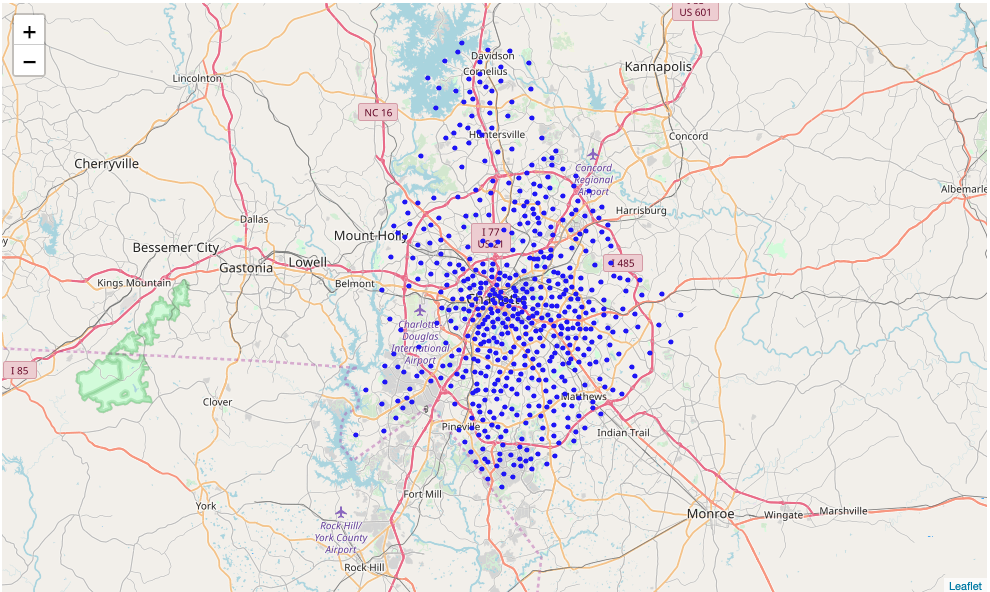
\includegraphics{img/m1.png}
\caption{Charlotte Map}
\end{figure}

    \hypertarget{after-clustering-by-median-household-income}{%
\subsubsection{After Clustering by Median Household
Income}\label{after-clustering-by-median-household-income}}

    \begin{figure}
\centering
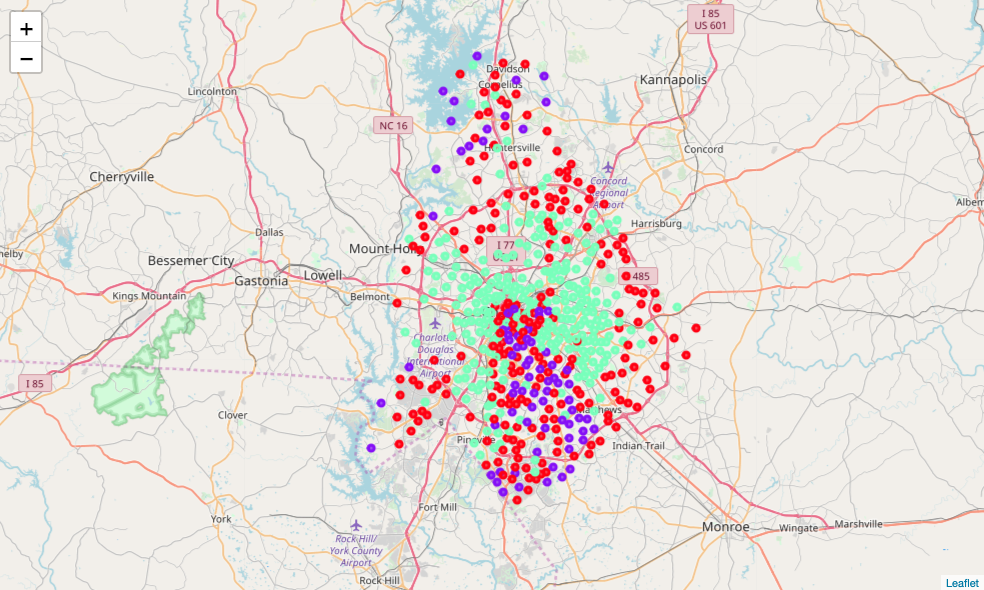
\includegraphics{img/m2.png}
\caption{Charlotte Map}
\end{figure}

    \hypertarget{and-here-we-see-the-average-for-each-cluster}{%
\subsubsection{And here we see the average for each
cluster}\label{and-here-we-see-the-average-for-each-cluster}}

    \begin{figure}
\centering
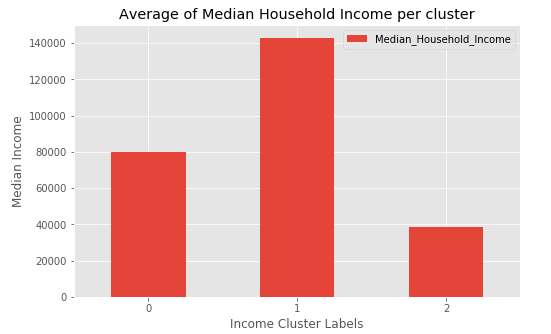
\includegraphics{img/income.png}
\caption{Charlotte Map}
\end{figure}

    \hypertarget{after-clustering-by-population-density}{%
\subsubsection{After Clustering by Population
Density}\label{after-clustering-by-population-density}}

    \begin{figure}
\centering
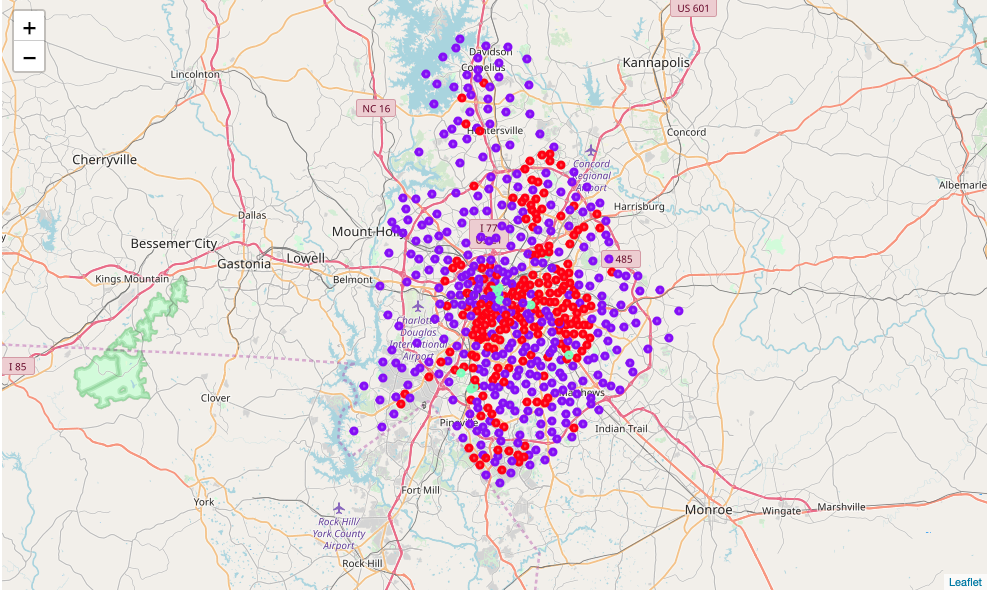
\includegraphics{img/m3.png}
\caption{Charlotte Map}
\end{figure}

    \hypertarget{and-here-we-see-the-average-for-each-cluster}{%
\subsubsection{And here we see the average for each
cluster}\label{and-here-we-see-the-average-for-each-cluster}}

    \begin{figure}
\centering
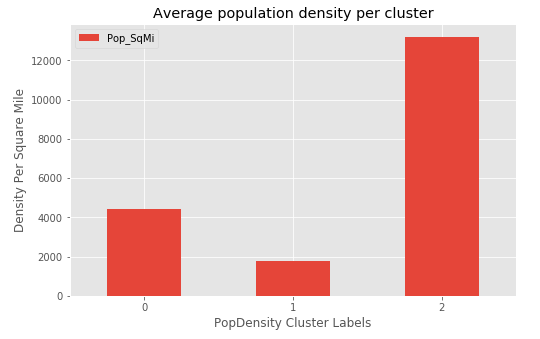
\includegraphics{img/density.png}
\caption{Charlotte Map}
\end{figure}

    \hypertarget{methodology}{%
\subsection{Methodology }\label{methodology}}

    The first step of our methodology was to collect location, demographic,
income and venues data for the City of Charlotte. We have collected and
preprocessed the data as a first step. We'll segment the data set two
different ways by Kmeans clustering. The first clustering method will be
by Household Median income and the second will be based on population
density per Census block i.e.~population per square mile. Afterwards
we'll use the clusters to create Wordclouds of the venues categories by
cluster. This will show us what kind of venues are near each type of
population area and help us gain better understanding about the City of
Charlotte.

    \hypertarget{analysis}{%
\subsection{Analysis }\label{analysis}}

    \hypertarget{income-clusters}{%
\subsubsection{Income Clusters}\label{income-clusters}}

    \hypertarget{income-cluster-label-0}{%
\paragraph{Income Cluster Label 0}\label{income-cluster-label-0}}

\begin{figure}
\centering
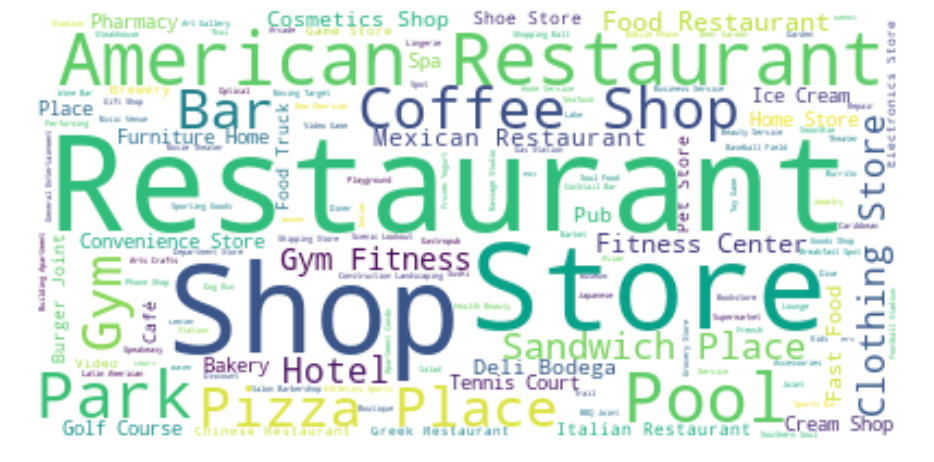
\includegraphics{img/m1c0.png}
\caption{Charlotte Map}
\end{figure}

\hypertarget{income-cluster-label-1}{%
\paragraph{Income Cluster Label 1}\label{income-cluster-label-1}}

\begin{figure}
\centering
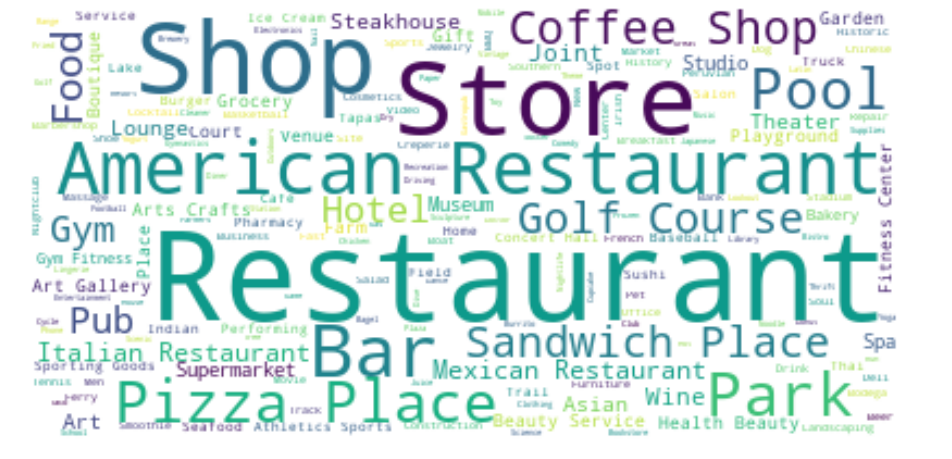
\includegraphics{img/m1c1.png}
\caption{Charlotte Map}
\end{figure}

\hypertarget{income-cluster-label-2}{%
\paragraph{Income Cluster Label 2}\label{income-cluster-label-2}}

\begin{figure}
\centering
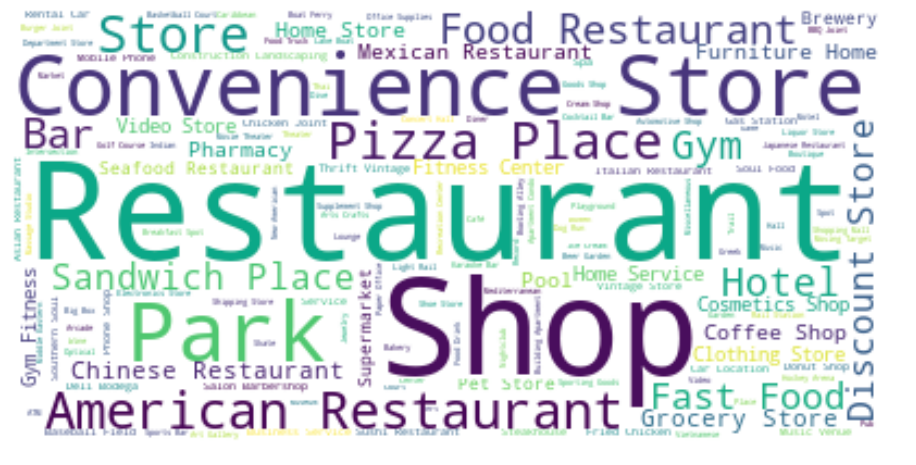
\includegraphics{img/m1c2.png}
\caption{Charlotte Map}
\end{figure}

    \hypertarget{density-cluster-clusters}{%
\subsubsection{Density Cluster
Clusters}\label{density-cluster-clusters}}

    \hypertarget{population-density-cluster-label-0}{%
\paragraph{Population Density Cluster Label
0}\label{population-density-cluster-label-0}}

\begin{figure}
\centering
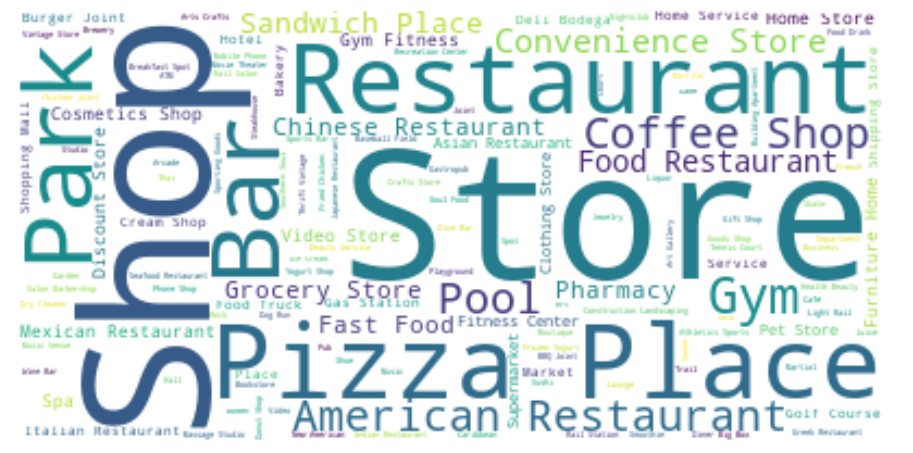
\includegraphics{img/m2c0.png}
\caption{Charlotte Map}
\end{figure}

\hypertarget{population-density-cluster-label-1}{%
\paragraph{Population Density Cluster Label
1}\label{population-density-cluster-label-1}}

\begin{figure}
\centering
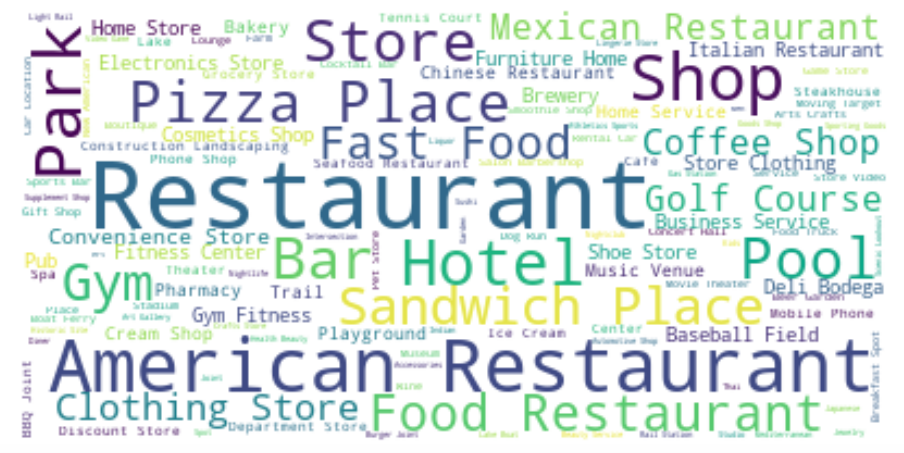
\includegraphics{img/m2c1.png}
\caption{Charlotte Map}
\end{figure}

\hypertarget{population-density-cluster-label-2}{%
\paragraph{Population Density Cluster Label
2}\label{population-density-cluster-label-2}}

\begin{figure}
\centering
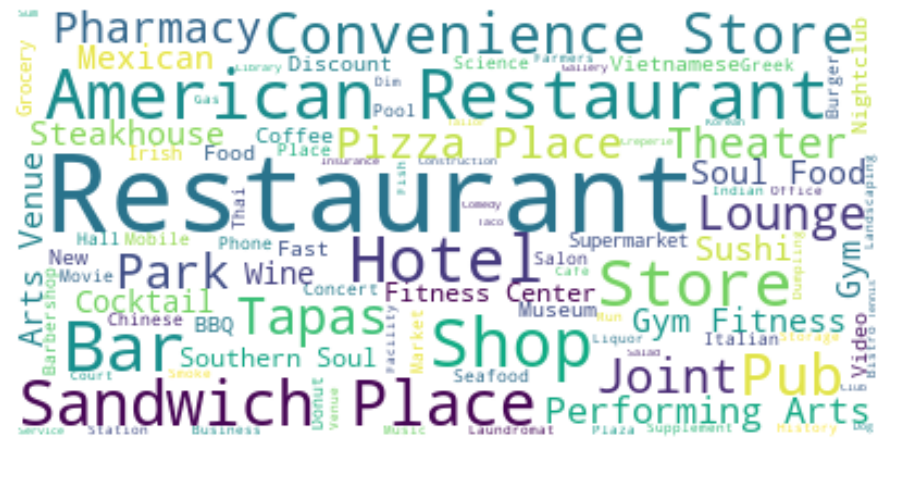
\includegraphics{img/m2c2.png}
\caption{Charlotte Map}
\end{figure}

    \hypertarget{results}{%
\subsection{Results }\label{results}}

    We were able to segment the City of Charlotte into 3 clusters by income
and population density. We observe the following trends based on each
clustering method:

\textbf{Income Clusters}

\begin{enumerate}
\def\labelenumi{\arabic{enumi}.}
\item
  Cluster Label 0 - Households with average income of 80,000. This is
  probably what we may call ``Middle Income''. We see that the venues
  near this group feature American and other Restaurants, Shopping,
  Stores, Coffee shops, Bar, Parks, Pools and Gyms.
\item
  Cluster Label 1 - Households with average income of above 140,000.
  We'll call this group ``Upper Income''. We see that the venues near
  this cluster group feature similar venues as Cluster 1, but we also
  see that we have Gold Courses near those households
\item
  Cluster Label 2 - Household with average income of 40,000. We'll call
  this group ``Lower Income''. We see that Restaurants are still
  prominent, but American Restaurants are not as popular there. We see a
  lot of Convenience stores, Shopping and Parks, but also Fast Food
  places.
\end{enumerate}

\textbf{Population Density Clusters}

\begin{enumerate}
\def\labelenumi{\arabic{enumi}.}
\item
  Cluster Label 0 - Medium Population Density with an average of around
  4,000 per square mile. We see a very strong trend for Shops, Stores
  and Pizza Places and fewer other venues comparitively.
\item
  Cluster Label 1 - Low Population Density with an average of less than
  2,000 per square mile. There is a better mix of venues in this cluster
  featuring Restaurants, Shopping, Hotels, Sandwitch Places, Fast Food
  and Parks.
\item
  Cluster Label 2 - High Population Density with an average of close to
  13,000 per square mile. This group features a lot more venues which we
  have not seen previously like Performing Arts, Theatre, Soul food,
  Arts Venue in addition to what we have learned to expect
  i.e.~Restaurants and Shops.
\end{enumerate}

    \hypertarget{conclusion}{%
\subsection{Conclusion }\label{conclusion}}

    Our investigation in the City of Charlotte revealed some interesting,
but probably expected results. We can find American Restaurants almost
anywhere in the city. Other Restaurants and Shopping is also easy to
come by. We find more Fast Food places and Convenience Stores compared
to other venues in lower income areas of the city. We also do see the
highest variety of venues and entertainment in the very high population
density areas of the city i.e.~downtown.

This notebook shows just 2 of the clustering methods, but many more are
possible with the available information.


    % Add a bibliography block to the postdoc
    
    
    
    \end{document}
